\documentclass[mat1, tisk]{fmfdelo}
\usepackage{amsmath}
\usepackage{graphicx}
\usepackage{hyperref}
% \usepackage[maxbibnames=99, articlein=false]{biblatex}
% \addbibresource{literatura.bib}


% \documentclass[fin1, tisk]{fmfdelo}
% Če pobrišete možnost tisk, bodo povezave obarvane,
% na začetku pa ne bo praznih strani po naslovu, …

%%%%%%%%%%%%%%%%%%%%%%%%%%%%%%%%%%%%%%%%%%%%%%%%%%%%%%%%%%%%%%%%%%%%%%%%%%%%%%%
% METAPODATKI
%%%%%%%%%%%%%%%%%%%%%%%%%%%%%%%%%%%%%%%%%%%%%%%%%%%%%%%%%%%%%%%%%%%%%%%%%%%%%%%

% - vaše ime
\avtor{Manca Murn}

% - naslov dela v slovenščini
\naslov{Metrična dimenzija leksikografskega produkta grafov}

% - naslov dela v angleščini
\title{The metric dimension of the lexicographic product of graphs}

% - ime mentorja/mentorice s polnim nazivom:
%   - doc.~dr.~Ime Priimek
%   - izr.~prof.~dr.~Ime Priimek
%   - prof.~dr.~Ime Priimek
%   za druge variante uporabite ustrezne ukaze
\mentor{prof.~dr.~Sandi Klavžar}
% \somentor{...}
% \mentorica{...}
% \somentorica{...}
% \mentorja{...}{...}
% \somentorja{...}{...}
% \mentorici{...}{...}
% \somentorici{...}{...}

% - leto diplome
\letnica{2024} 

% - povzetek v slovenščini
%   V povzetku na kratko opišite vsebinske rezultate dela. Sem ne sodi razlaga
%   organizacije dela, torej v katerem razdelku je kaj, pač pa le opis vsebine.
\povzetek{...}

% - povzetek v angleščini
\abstract{... }

% - klasifikacijske oznake, ločene z vejicami
%   Oznake, ki opisujejo področje dela, so dostopne na strani https://www.ams.org/msc/
\klasifikacija{..., ...}

% - ključne besede, ki nastopajo v delu, ločene s \sep
\kljucnebesede{...\sep ...}

% - angleški prevod ključnih besed
\keywords{...\sep ...} % angleški prevod ključnih besed

% - angleško-slovenski slovar strokovnih izrazov
\slovar{
% \geslo{angleški izraz}{slovenski izraz}
% ...
}

% - ime datoteke z viri (vključno s končnico .bib), če uporabljate BibTeX
\literatura{literatura.bib}

%%%%%%%%%%%%%%%%%%%%%%%%%%%%%%%%%%%%%%%%%%%%%%%%%%%%%%%%%%%%%%%%%%%%%%%%%%%%%%%
% DODATNE DEFINICIJE
%%%%%%%%%%%%%%%%%%%%%%%%%%%%%%%%%%%%%%%%%%%%%%%%%%%%%%%%%%%%%%%%%%%%%%%%%%%%%%%

% naložite dodatne pakete, ki jih potrebujete
% \usepackage{...}

% deklarirajte vse matematične operatorje, da jih bo LaTeX pravilno stavil
% \DeclareMathOperator{\...}{...}

% vstavite svoje definicije ...
% \newcommand{\...}{...}
\newcommand{\1}{(1, 1, \ldots, 1)}
\newcommand{\2}{(2, 2, \ldots, 2)}



%%%%%%%%%%%%%%%%%%%%%%%%%%%%%%%%%%%%%%%%%%%%%%%%%%%%%%%%%%%%%%%%%%%%%%%%%%%%%%%
% ZAČETEK VSEBINE
%%%%%%%%%%%%%%%%%%%%%%%%%%%%%%%%%%%%%%%%%%%%%%%%%%%%%%%%%%%%%%%%%%%%%%%%%%%%%%%

\begin{document}

\section{Uvod}
V decembru leta 2010 sta v razmaku 17 dni nastala dva različna članka z enakim naslovom - 
\textit{''The metric dimension of the lexicographic product of graph''}. Avtorji obeh člankov 
niso vedeli za delo drugega in so se teme lotili na dva posvem različna načina. V tem diplomskem 
seminarju si bomo ogledali pojma metrične in sosedske dimenzije grafa in njune osnovne lastnosti, 
ter povezave med njima, definirali bomo leksikografski produkt grafov ter povzeli 
glavne rezultate o metrični dimenziji leksikografskega produkta iz obeh člankov.


%%%%%%%%%%%%%%%%%%%%%%%%%%%%%%%%%%%%%%%%%%%%%%%%%%%%%%%%%%%%%%%%%%%%%%%%%%%%%%%
%%%%%%%%%%%%%%%%%%%%%%%%%%%%%%%%%%%%%%%%%%%%%%%%%%%%%%%%%%%%%%%%%%%%%%%%%%%%%%%


\subsection{Osnovni pojmi} \label{ss:osnovni_pojmi}
Za začetek ponovimo nekaj osnovnih definicij in oznak iz teorije grafov, ki jih bomo potrebovali 
za razumevanje tega diplomskega seminarja. 

\begin{definicija} \label{def:graf}
    Graf $G$ je urejen par $(V(G), E(G)),$ kjer je $V(G)$ množica vozlišč in $E(G)$ 
    podmnožica v $\binom{V(G)}{2},$ ki vsebuje povezave grafa.
\end{definicija}

Če je $V(G)$ končna množica, je $G$ končen graf. Število $|V(G)|$ imenujemo red grafa. 
Če je med dvema različnima vozliščema največ ena povezava in nobeno vozlišče ni povezano samo 
s seboj, pravimo, da je graf enostaven. Povezave med vozlišči $\{u, v\}$ bomo zaradi preglednosti
pisali kar $uv$. Vozlišči $v, u \in G$ sta sosedni, če $uv \in E(G).$ 
Sosednost je ekvivalenčna relacija, zato sosedni vozlišči označimo $u \sim v.$ Če $w, x \in V(G)$ 
nista sosedni pa pišemo $w \not \sim x.$

\begin{definicija} \label{def:sosescina}
    Naj bo $G$ graf in $v \in V(G)$. Množico 
    $$N(v) = \{u \in V(G) \, | \,vu \in E(G) \}$$ imenujemo soseščina vozlišča $v$.

    Stopnja vozlišča je ${\rm deg}(u) = |N(u)|.$
\end{definicija}


\begin{definicija} \label{def:komplement}
    Komplement grafa $G$, je graf $\overline{G},$ za katerega velja $V(G) = V(\overline{G})$ in 
    $$\forall u,v \in V(\overline{G}): uv E(\overline{G}) \Leftrightarrow uv \not \in E(G).$$
\end{definicija}

Sprehod v grafu $G$ je zaporedje vozlišč $v_1, v_2, \ldots v_k$ iz $V(G)$, tako da je 
$\forall i : v_i, v_{i+1} \in E(G).$ Sprehod je enostaven, če vsebuje sama različna vozlišča.
Graf je povezan, če med vsakima dvema različnima vozliščema obstaja sprehod. Na povezanem
grafu lahko definiramo razdaljo med vozliščema.

\begin{definicija} \label{def:razdalja}
    Razdalja med dvema vozliščema $u, v \in V(G)$ je dolžina najkrajšega sprehoda in jo 
    označujemo z $d_{G}(u, v).$ 
\end{definicija}

Naslednja trditev o razdaji med vozlišči je očitna.

\begin{trditev} \label{trd:nicelna_razdalja}
    Za povezan graf $G$ in poljubni vozlišči $v, w \in V(G)$ velja:
    $$ d_{G}(v, w) = 0 \Leftrightarrow v=w.$$
\end{trditev} 

\begin{definicija} \label{def:premer}
    Premer povezanega grafa $G$ označujemo z ${\rm diam}(G)$ in je enak največji razdalji med vozlišči.
    Torej $${\rm diam}(G) = \underset{v, u \in V(G)}{\max} d_{G}(u, v).$$
\end{definicija}

Iz definicije očitno sledi, da za poljubni dve vozlišči $u, v$ iz povezanega grafa $G$
velja $0 \leq d_G (u, v) \leq {\rm diam}(G).$

\begin{definicija} \label{def:podgraf}
    Graf $H$ je podgraf grafa $G$, če velja $V(H) \subseteq V(G)$ in 
    $E(H) \subseteq E(G)$.

    Podgraf $H$ je induciran, če velja 
    $\forall u, v \in V(H) : uv \in E(G) \Rightarrow E(H)$.
\end{definicija}

\begin{definicija} \label{def:komponenta}
Komponenta grafa je povezan podgraf, ki ni del nobenega večjega povezanega podgrafa. 
\end{definicija}
%nerazumljiv komentar

Povezan graf ima seveda samo eno komponento. Definirajmo še operacijo spojitve grafov.

\begin{definicija} \label{def:spoj}
    Spoj grafov $G$ in $H$, je graf $G + H$, za katerega velja $V(G + H) = V(G) \cup V(H)$ 
    in $E(G + H)  = E(G) \cup E(H) \cup \{ uv \;  | \;  u \in V(G) \land v \in V(H) \}.$
\end{definicija}

Poglejmo še nekaj primerov osnovnih razredov grafov:
\begin{itemize} \label{razredi_grafov}
    \item Graf brez povezav na $n$ vozliščih, ki ga označujemo z $N_n$, nima nobenih povezav. 
    \item Polni graf na $n$ vozliščih, ki ga označujemo s $K_n$, ima vse možne povezave.
    \item Polni dvodelni graf $K_{n, m}$ ima množico 
    vozlišč $V(K_{n,m}) = \{ v_{1, 1}, v_{1, 2}, \ldots , v_{1, n},  \allowbreak v_{2, 1}, v_{2, 2}, \ldots , v_{2, m} \}$
    in povezave $E(K_{n, m}) = \{ v_{1, i} v_{2, j} \; | \; i, j \in \{ 1, 2, \ldots , m \} \}.$ 
    \item  Polni $t$-delni graf, ki ga označujemo s $K_{m_1, \ldots, m_t}$, ima množico 
    vozlišč enako $V(K_{m_1, \ldots, m_t}) = \{ v_{1, 1}, v_{1, 2}, \ldots , v_{1, m_1}, 
     v_{2, 1}, v_{2, 2}, \ldots , v_{2, m_2}, \ldots , v_{t, 1}, v_{t, 2}, \ldots , v_{t, m_t}\}$,
    množica povezav pa je $E(K_{m_1, \ldots, m_t}) = \{  v_{a, i} v_{b, j} \; | \; a \neq b \land \; 
    i, j \in \{ 1, 2, \ldots , m \} \}.$
    \item Zvezda na $n$ vozliščih je poseben primer polnega dvodelnega grafa in jo označujemo
    s $S_{n-1} = K_{1, n-1}$
    \item Pot na $n$ vozliščih, kjer je $n \geq 2$, ki jo označujemo s $P_n$, ima množico povezav 
    $E(P_n) = \{ v_1 v_2 , v_2 v_3 , \ldots , v_{n-1} v_n\}.$
    \item Cikel na $n$ vozliščih, kjer je $n \geq 3$, dobimo tako, da grafu $P_n$ dodamo povezavo $v_n v_1$. 
    Označimo ga s $C_n$.
    \item Polni razcepljeni graf na $k+l$ vozliščih je enak spoju poti in grafa brez povezav ter ga 
    označujemo s $F_{k,l} = N_k + P_l.$
    %fan graph
    \item Drevo je povezan graf, ki ne vsebuje nobenega cikla.
\end{itemize}

\begin{opomba}
    Očitno velja $K_1 = N_1.$ To je graf s samo enim vozliščem. Običajno ga bomo
    označevali s $K_1.$
\end{opomba}


%%%%%%%%%%%%%%%%%%%%%%%%%%%%%%%%%%%%%%%%%%%%%%%%%%%%%%%%%%%%%%%%%%%%%%%%%%%%%%%
%%%%%%%%%%%%%%%%%%%%%%%%%%%%%%%%%%%%%%%%%%%%%%%%%%%%%%%%%%%%%%%%%%%%%%%%%%%%%%%
%%%%%%%%%%%%%%%%%%%%%%%%%%%%%%%%%%%%%%%%%%%%%%%%%%%%%%%%%%%%%%%%%%%%%%%%%%%%%%%
%%%%%%%%%%%%%%%%%%%%%%%%%%%%%%%%%%%%%%%%%%%%%%%%%%%%%%%%%%%%%%%%%%%%%%%%%%%%%%%


\section{Metrična dimenzija grafa} \label{s:mdim}

motivacija TODO

%%%%%%%%%%%%%%%%%%%%%%%%%%%%%%%%%%%%%%%%%%%%%%%%%%%%%%%%%%%%%%%%%%%%%%%%%%%%%%%
%%%%%%%%%%%%%%%%%%%%%%%%%%%%%%%%%%%%%%%%%%%%%%%%%%%%%%%%%%%%%%%%%%%%%%%%%%%%%%%


\subsection{Definicija} \label{ss:def_mdim}

Metrična dimenzija grafa je najmanjše število vozlišč grafa, ki jih potrebujemo, da
vsa vozlišča v grafu razlikujemo med sabo zgolj s pomočjo razdalj do izbranih vozlišč.
Formalno to povemo takole:

\begin{definicija} \label{def:mdim}
    Naj bo $G$ povezan graf. 
    \begin{itemize}
        \item Naj bo $W = \{ w_1, \ldots , w_k  \} \subseteq V(G)$ neprazna podmnožica vozlišč. 
        Vektor $r_W(v) = (d(v, w_1), \ldots, d(v, w_k))$ imenujemo metrična 
        predstavitev vozlišča $v \in V(G)$ s podmnožico $W$.
        \item Neprazna podmnožica $R \subseteq V(G)$ je rešljiva,
        če $\forall u, v \in V(G): u \neq v \implies r_R(v) \neq r_R(u)$.
        \item Najmanjša rešljiva množica grafa $G$ se imenuje metrična baza. Njeno velikost imenujemo 
        metrična dimenzija in jo označimo z $\beta(G).$
    \end{itemize}
\end{definicija}

Za lažje razumevanje si poglejmo nekaj lahkih osnovnih primerov.

\begin{primer} \label{pr:mdim_pot}
Označimo vozlišča poti z $v_1, v_2, \ldots, v_n$, kot je prikazano na spodnji sliki \ref{fig:pot}. 
Izberimo podmnožico $W = \{v_1\} \subseteq V(G).$ Metrične predstavitve vozlišč grafa $P_n$, 
glede na $W$, so potem sledeče:
\begin{align*}
    r_W(v_1) = d(v_1, v_1) & = 0 \\
    r_W(v_2) = d(v_2, v_1) & = 1 \\
    & \dots \\
    r_W(v_{n-1}) = d(v_{n-1}, v_1) & = n-2 \\
    r_W(v_n) = d(v_n, v_1) & = n-1.
\end{align*}

Vidimo, da so metrične predstavitve vseh vozlišč med seboj različne. Sledi, da je $W$ 
rešljiva množica. Ker je njena velikost enaka $1$ in je to najmanjša možna neprazna podmnožica 
vozlišč, je torej metrična dimenzija grafa poti poljubne dolžine enaka $\beta(P_n) = 1.$

\begin{figure}[h]
    \centering
    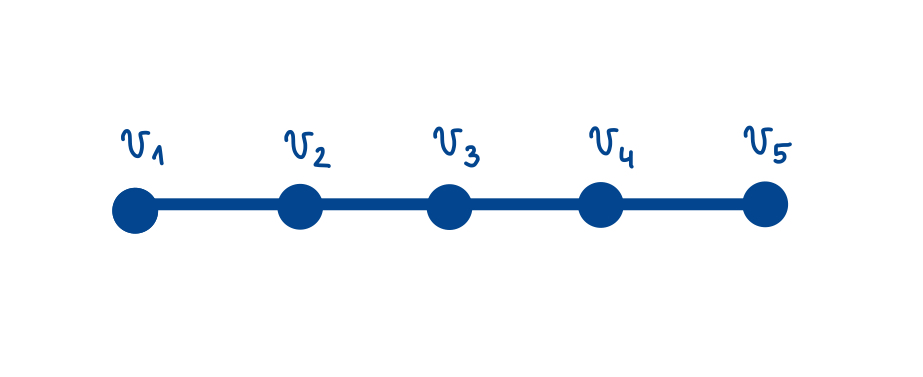
\includegraphics[width=0.6\textwidth]{IMG_pot.jpg}
    \caption{Graf $P_5$}
    \label{fig:pot}
\end{figure}

\end{primer}


\begin{primer}\label{pr:mdim_cikel}
    Označimo vozlišča cikla z $v_1, v_2, \ldots, v_n$, kot je prikazano na sliki \ref{fig:cikel}. 
    Izberimo podmnožico $W = \{ v_1, v_2 \} \subseteq V(G).$ Metrične predstavitve vozlišč grafa $C_n$, 
    glede na $W$, so potem sledeče:
    \begin{align*}
        r_W(v_1) = (d(v_1, v_1), d(v_1, v_2)) & = (0, 1) \\
        r_W(v_2) = (d(v_2, v_1), d(v_2, v_2)) & = (1, 0) \\
        & \dots \\
        r_W(v_{n-1}) = (d(v_{n-1}, v_1), d(v_{n-1}, v_2)) & = (2, 3) \\
        r_W(v_n) = (d(v_n, v_1), d(v_n, v_2)) & = (1, 2)
    \end{align*}
    
    Zopet vidimo, da so metrične predstavitve vseh vozlišč med seboj različne. Če bi vzeli 
    množico s samo enim vozliščem, bi imeli po dve vozlišči enako metrično prestavitev.
    $W$  je torej najmanjša rešljiva množica, njena velikost pa je enaka $2$. Metrična 
    dimenzija poljubno velikega cikla je enaka $\beta(C_n) = 2.$

    \begin{figure}[h]
        \centering
        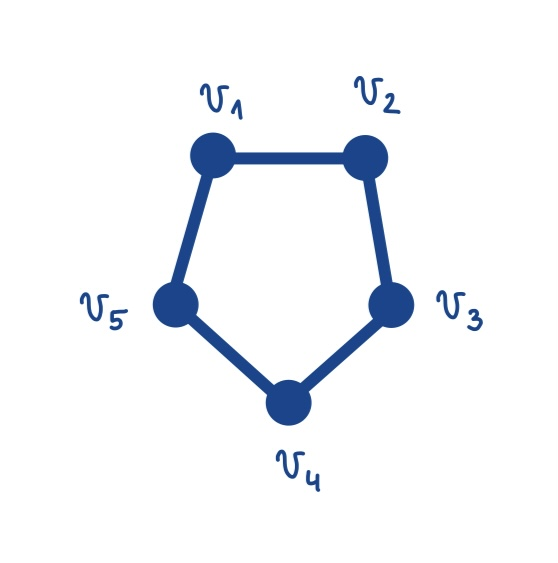
\includegraphics[width=0.4\textwidth]{IMG_cikel.jpg}
        \caption{Graf $C_5$.}
        \label{fig:cikel}
    \end{figure}

\end{primer}


\begin{primer}\label{pr:mdim_poln}
    Označimo vozlišča polnega grafa z $v_1, v_2, \ldots, v_n$, kot je prikazano na sliki \ref{fig:polni}. 
    Izberimo podmnožico $W = \{ v_1, v_2, \ldots , v_{n-1} \} \subseteq V(G).$ 
    Metrične predstavitve vozlišč grafa $K_n$, glede na $W$, so potem sledeče:
    \begin{align*}
        r_W(v_1) = (d(v_1, v_1), d(v_1, v_2), \ldots , d(v_1, v_{n-1})) & = (0, 1, \ldots , 1) \\
        r_W(v_2) = (d(v_2, v_1), d(v_2, v_2), \ldots , d(v_2, v_{n-1})) & = (1, 0, \ldots , 1) \\
        & \dots \\
        r_W(v_{n-1}) = (d(v_{n-1}, v_1), d(v_{n-1}, v_2), \ldots , d(v_{n-1}, v_{n-1})) & = (1, 1, \ldots , 0) \\
        r_W(v_n) = (d(v_n, v_1), d(v_n, v_2), \ldots ,  d(v_n, v_{n-1})) & = (1, 1, \ldots , 1)
    \end{align*}
    
    Zopet vidimo, da so metrične predstavitve vseh vozlišč med seboj različne. Vsako 
    vozlišče ima na $i$ - ti komponenti metrične predstavitve $0$ in povsod drugje $1$, 
    z izjemo vozlišča $v_n$, ki ima povsod $1$. Če bi iz $W$ izvzeli poljubno vozlišče $v_i$, 
    bi imeli vozlišči $v_i$ in $v_n$ enaki metrični predstavitvi. $W$  je torej najmanjša rešljiva množica, 
    njena velikost pa je $n-1$. Metrična dimenzija poljubno velikega polnega grafa je enaka 
    $\beta(K_n) = n-1.$

    \begin{figure}[h]
        \centering
        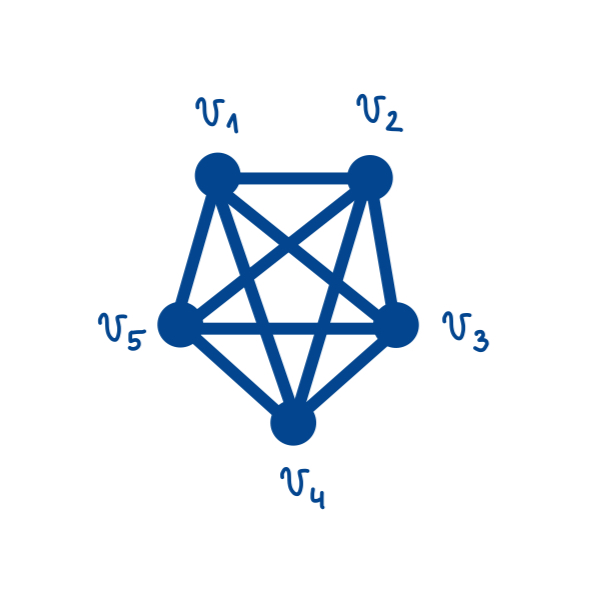
\includegraphics[width=0.4\textwidth]{IMG_polni.jpg}
        \caption{Graf $K_5$.}
        \label{fig:polni}
    \end{figure}

\end{primer}

%%%%%%%%%%%%%%%%%%%%%%%%%%%%%%%%%%%%%%%%%%%%%%%%%%%%%%%%%%%%%%%%%%%%%%%%%%%%%%%
%%%%%%%%%%%%%%%%%%%%%%%%%%%%%%%%%%%%%%%%%%%%%%%%%%%%%%%%%%%%%%%%%%%%%%%%%%%%%%%

\subsection{Sosedska dimenzija grafa} \label{ss:sdim}
V nekaterih primerih si bomo pri obravnavanju metrične dimenzije pomagali tudi s pojmom 
sosedske dimenzije. 

Pri sosedski dimenziji zopet iščemo podmnožico vozlišč, s pomočjo katerih bomo lahko vsa 
vozlišča v grafu med sabo razlikovali, vendar tokrat ne s pomočjo razdalje, pač pa s 
pomočjo relacije sosednosti. 

Definirajmo preslikavo  $a: V(G) \times V(G) \rightarrow \mathbb{N}$ takole:  
\begin{equation} \label{eq:fja_a} 
    a(v, w) = 
    \begin{cases}
        0; & v = w \\
        1; & v \sim w \\
        2; & v \not\sim w
    \end{cases} 
\end{equation} 

Sedaj lahko zapišemo naslednjo definicijo.

\begin{definicija} \label{def:sdim}
    Naj bo $G$ poljuben graf. 
    \begin{itemize}
        \item Naj bo $W = \{ w_1, \ldots , w_k  \} \subseteq V(G)$ neprazna podmnožica vozlišč. 
        Vektor $s_W(v) = (a(v, w_1), \ldots, a(v, w_k))$ imenujemo 
        sosedska predstavitev vozlišča $v \in V(G)$ s podmnožico $W$.
        \item  Podmnožica vozlišč $S \subseteq V(G)$ je sosedsko rešljiva,
        če $\forall u, v \in V(G): u\neq v \implies s_S(v) \neq s_S(u)$.
        \item Najmanjša sosedsko rešljiva množica grafa $G$ se imenuje sosedska baza. 
        Njeno velikost imenujemo sosedska dimenzija in jo označimo z $\mu (G).$
    \end{itemize}    
\end{definicija}


%%%%%%%%%%%%%%%%%%%%%%%%%%%%%%%%%%%%%%%%%%%%%%%%%%%%%%%%%%%%%%%%%%%%%%%%%%%%%%%


\subsubsection{Lastnosti sosedske dimenzije} \label{sss:lastnosti_sdim}

\begin{trditev} \label{trd:lastnosti_sdim}
    Naj bo $G$ povezan graf. Potem velja:
    \begin{enumerate}
        \item $\mu(G) \geq \beta(G)$.
        \item ${\rm diam}(G) = 2 \Rightarrow \mu(G) = \beta(G).$
        \item $\mu(G) = \mu(\overline{G}).$
        \item $\mu(G) = 1 \Leftrightarrow G \in \{P_1, P_2, P_3, \overline{P_2}, \overline{P_3}\}.$
        \item $\mu(G) = n - 1 \Leftrightarrow G \in \{K_n, \overline{K_n}\}.$
    \end{enumerate}
\end{trditev}

\begin{dokaz}
    TODO
\end{dokaz}

% primeri
%%%%%%%%%%%%%%%%%%%%%%%%%%%%%%%%%%%%%%%%%%%%%%%%%%%%%%%%%%%%%%%%%%%%%%%%%%%%%%%
%%%%%%%%%%%%%%%%%%%%%%%%%%%%%%%%%%%%%%%%%%%%%%%%%%%%%%%%%%%%%%%%%%%%%%%%%%%%%%%


\subsection{Lastnosti metrične dimenzije} \label{s:lastnosti_mdim}

Oglejmo si nekaj osnovnih ugotovitev o metrični dimenziji. Iz primera \ref{pr:mdim_pot}
lahko hitro razberemo, da metrična baza ni nujno enolično določena. Za $W$ bi lahko 
vzeli tudi vozlišče $v_n$ in prišli do enakega rezultata. 
Poiščimo sedaj najbolj splošno omejitev za metrično dimenzijo.

\begin{trditev} \label{trd:cela_resljiva}
Za povezan graf $G$, je $V(G)$ rešljiva množica. Še več, za poljubno vozlišče $v_i \in V(G)$
je $W_i = V(G) \setminus \{ v_i\}$ rešljiva množica.
\end{trditev}

\begin{dokaz}
Naj bo $G$ povezan in $|V(G)|= n$. Označimo vozlišča z $v_1, \ldots, v_n$.
Upoštevajoč trditev \ref{trd:nicelna_razdalja} hitro opazimo, da velja 
$\forall j \in \{ 1, 2, \ldots , i - 1, i + 1, \ldots , n\}:$ vozlišče $v_j$ ima natanko $j$-to komponento 
metrične predstavitve glede na $W_i$ enako $0$. Vozlišče $v_i$ pa je edino, ki ima vse komponente 
različne od $0.$ Sledi $\forall u, v \in V(G): u \neq v \Rightarrow r_{W_i}(v) \neq r_{W_i}(u)$, 
torej je $W_i$ rešljiva množica.
Če rešljivi množici dodamo še kako vozlišče, je tudi slednja očitno rešljiva. Torej je tudi 
$V(G) = W_i \cup \{ v_i\}$  rešljiva.
\end{dokaz}

Metrična baza povezanega grafa torej vselej obstaja.

\begin{posledica} \label{po:groba_omejitev_mdim}
    Za povezan graf $G$ velja 
    $$1 \leq \beta(G) \leq |V(G)| - 1. $$
\end{posledica}

\begin{opomba} \label{op:zadostno_preverjanje}
    Če za neko množico $S \subseteq V(G)$ preverjamo, če je rešljiva, je dovolj preveriti metrične 
    predstavitve vozlišč $v \in V(G) \setminus S.$ Vozlišča iz $S$ bodo imela natanko eno komponento 
    vektorja enako nič. 
\end{opomba}

\begin{lema} \label{lema:vozlisce_max_deg_1}
    Naj bo $G$ povezan graf in $|V(G)| = n,$ ter naj bodo $u_1, \ldots, u_k \in V(G)$ vozlišča stopnje $n-1.$
    Potem metrična baza v $G$ vsebuje vsaj $k-1$ vozlišč stopnje $n-1.$
\end{lema}

\begin{dokaz}
    Denimo, da je $R$ metrična baza povezanega grafa $G$, ki vsebuje manj kot $k-1$ vozlišč stopnje $n-1$. 
    Potem imajo vozlišča stopnje $n-1$, ki niso vsebovana v $R$, metrično predstavitev glede na $R$ enako 
    $\1$ in sledi, da $R$ ne more biti metrična baza. 
\end{dokaz}

\begin{lema} \label{lema:vozlisce_max_deg_2}
    Naj bo $G$ povezan graf in $|V(G)| = n,$ ter naj bo $u \in V(G)$ vozlišče stopnje $n-1.$
    Potem obstaja metrična baza v $G$, ki ne vsebuje vozlišča $u.$
\end{lema}

\begin{dokaz}
    Naj bo $G$ povezan graf reda $n$, $u$ vozlišče stopnje $n-1$ in $R$ metrična baza.
    \begin{enumerate}
        \item Če $u \notin R$ smo končali.
        \item Denimo, da $u \in R.$ Želimo si $u$ zamenjati z nekim drugim vozliščem grafa. 
         Označimo $R = \{v_1, v_2, \ldots, v_k, u\}$ in $V(G) = R \cup \{v_{k+1}, v_{k+3}, \ldots, v_n \}.$
         Velja:
         \begin{align*}
            r_R(v_{k+1}) & = (d(v_{k+1}, v_1), d(v_{k+1}, v_2), \ldots, 1) \\
            r_R(v_{k+2}) & = (d(v_{k+2}, v_1),  d(v_{k+2}, v_2), \ldots, 1) \\
            & \dots \\
            r_R(v_n)  & = (d(v_n, v_1), d(v_n, v_2), \ldots, 1).
        \end{align*}
        Vidimo, da se morajo metrične predstavitve vozlišč, ki niso vsebovana v $R$, razlikovati v prvih $k$
        komponentah. 
        
        Denimo, da obstaja vozlišče, ki ima metrično predstavitev enako $ \1.$ Po definiciji je tako največ eno in 
        BŠS naj bo to $v_{k+1}$.
        Vzemimo $R' = (R \setminus \{u\} ) \cup  \{v_{k+1}\}$.
        Metrične predstavitve vozlišč $v_{k+2}, \ldots v_n$ glede na $R'$ se še vedno razlikujejo v prvih $k$ komponentah,
        $u$ pa je edino voszlišče z metrično predstavitvijo $\1.$ $R'$ je torej metrična baza.

        Če nobeno vozlišče nima metrične predstavitve glede na $R$ enako $\1,$ lahko $u$ zamenjamo s poljubnim drugim
        vozliščem, ki še ni vsebovano v $R$. 
    \end{enumerate}
\end{dokaz}

    

V splošnem je iskanje metrične dimenzije grafa NP-poln problem. Za nekatere vrste grafov
pa lahko najdemo eksplicitne formule za njen izračun.

\begin{trditev} \label{trd:mdim_polni_pot}
    Naj bo $G$ povezan graf in $|V(G)| = n \geq 2.$ Potem velja:
    \begin{enumerate}
        \item $G = K_n \; \Leftrightarrow \; \beta(G) = n - 1.$
        \item $G = P_n \; \Leftrightarrow \; \beta(G) = 1.$
    \end{enumerate} 
\end{trditev}

\begin{dokaz}
    Implikacijo v desno stran za obe točki smo že pokazali v \ref{pr:mdim_pot} in 
    \ref{pr:mdim_poln}.
    \begin{enumerate}
        \item $\Leftarrow$ 
        Recimo, da imamo povezan graf $G$ na $n$ vozliščih z $\beta(G) = n - 1.$ Označimo metrično bazo
        z $W = \{v_1, v_2, \ldots, v_{n-1}\}$ in $V(G) = W \cup \{v_n\}$. 
        
        Če odstranimo poljubno vozlišče $v_i$ iz množice $W$, morata obstajati vsaj dve vozlišči, katerih metrični 
        predstavitvi se ne razlikujeta glede na $W' = W \setminus \{v_i \}$ - v nasprotnem primeru $W$ ni bila metrična baza. 
        Še vedno se metrična predstavitev vsakega vozlišča vsebovanega v $W'$, glede na $W'$, razlikuje od vseh ostalih. 
        Sledi $r_{W'}(v_i) = r_{W'}(v_n)$.
        Ker smo vzeli poljubno vozlišče iz množice $W$, lahko enako ponovimo še z vsemi ostalimi. Sledi 
        $$\forall v_j \in W:  r_{W \setminus \{v_j\}}(v_j)= r_{W \setminus \{v_j\}}(v_n).$$
        Označimo $deg(v_n) = k, \; 1 \leq k \leq n-1$. Metrične predstavitve vseh vozlišč glede na $W$ so potem sledeče:
        \begin{align*}
            r_W(v_1) & = (0, 1, \ldots 1, d(v_n, v_{k+1}), \ldots,d(v_n, v_{n-1})) \\
            r_W(v_2) & = (1, 0, \ldots 1, d(v_n, v_{k+1}), \ldots,d(v_n, v_{n-1}))\\
            & \dots \\
            r_W(v_k)  & = (1, 1, \ldots 0, d(v_n, v_{k+1}), \ldots,d(v_n, v_{n-1}))\\
            r_W(v_{k+1}) & = (1, 1, \ldots 1, 0, \ldots,d(v_n, v_{n-1})) \\
            & \dots \\
            r_W(v_{n - 1}) & = (1, 1, \ldots 1, d(v_n, v_{k+1}), \ldots, 0) \\
            r_W(v_n)  & = (1, 1, \ldots 1, d(v_n, v_{k+1}), \ldots,d(v_n, v_{n-1})).
        \end{align*}
        Ker je $G$ povezan, mora obstajati vsaj eno vozlišče $v_i,$ da velja $d(v_i, v_{k+1}) = 1.$ Potem sledi
        $$d(v_1, v_{k+1}) = d(v_2, v_{k+1}) = \ldots d(v_k, v_{k+1}) = d(v_{k+2}, v_{k+1}) = \ldots d(v_n, v_{k+1}) = 1.$$
        Podobno velja za $v_{k+2}, v_{k+3}, \ldots, v_{n-1}.$ Sledi, da so vsa vozlišča stopnje $n-1$ in $G = K_n.$
        
        \item $\Leftarrow$
        Recimo, da imamo povezan graf $G$ na $n$ vozliščih z $\beta(G) = 1.$ Sledi, da obstaja neka 
        metrična baza $W = \{ w \}.$ Označimo $V(G) = \{ v_1, v_2, \ldots , v_{n-1}, w\}.$ Sedaj mora 
        veljati, da so števila 
        $$ d(v_1, w),  d(v_2, v_1), \ldots, d(v_{n-1}, w), d(w, w) $$
        paroma različna. Vemo $d(w, w) = 0$. Ker je $G$ povezan, mora obstajati vsaj eno vozlišče, 
        ki je sosednje z $w$. BSŠ naj bo $v_{n-1} \sim w$. Torej je $d(v_{n-1}, w) = 1$ in sledi, 
        da nobeno drugo vozlišče ni sosednje z $w$. Zopet zaradi povezanosti grafa obstaja vozlišče 
        sosednje z $v_{n-1},$ ki je različno od $w$. Recimo, da je to $v_{n-2}$, za katerega sedaj 
        velja $d(v_{n-2}, w) = 2.$ Spet je to edino takšno vozlišče. Nadaljujemo podobno, 
        dokler ne pridemo do $v_1.$ Dobimo graf $P_n.$
    \end{enumerate}
\end{dokaz}


\begin{trditev} \label{trd:mdim_spojev}
    Naj bo $n\geq 4$, potem velja:
    \begin{enumerate}
        \item $n \neq 6 \; \Rightarrow \; \beta(C_n + K_1) = 
        \Bigl \lfloor \frac{2n + 2}{5}\Bigr \rfloor$.
        \item $n \neq 6 \; \; \Rightarrow \; \beta(P_n + K_1) = 
        \Bigl \lfloor \frac{2n + 2}{5}\Bigr \rfloor$.
    \end{enumerate}
\end{trditev}

\begin{dokaz}
    TODO
\end{dokaz}

\begin{opomba}
    Za manjše $n$ velja:
    \begin{itemize}
        \item $C_3 + K_1 = K_4 \Rightarrow \beta(C_3 + K_1) = 3.$
        \item $P_2 + K_1 = C_3 \Rightarrow \beta(P_2 + K_1) = 2.$
        \item $\beta(P_3 + K_1) = 2.$
    \end{itemize}
    
\end{opomba}
%v opombo lahko  zapišem kaj se zgodi špri n = 1, 2, 3
%zakaj za 6 ne velja?


%%%%%%%%%%%%%%%%%%%%%%%%%%%%%%%%%%%%%%%%%%%%%%%%%%%%%%%%%%%%%%%%%%%%%%%%%%%%%%%


\subsubsection{Metrična dimenzija in premer grafa} \label{ss:mdim_premer}

Ni presenetljivo, da lahko najdemo povezavo med metrično dimenzijo in premerom grafa.

\begin{trditev}\label{trd:groba_meja_mdim_premer}
    Naj bo $G$ povezan graf in $|V(G)| = n$. Potem velja naslednja povezava:
    $$n \leq ({\rm diam}(G))^{\beta (G)} + \beta (G). $$
\end{trditev}

\begin{dokaz}
    Naj bo $R$ metrična baza grafa $G$, torej $|R| = \beta(G).$ Zanima nas, največ koliko 
    vozlišč ima lahko tak graf. Vozlišča iz množice $R$ bodo imela natanko eno 
    komponento metrične predstavitve enako nič, tako se bodo te razlikovale med sabo in od
    vseh ostalih. Če vzamemo vozlišče $v \notin R$, pa velja sledeče:
    $$\forall r_i \in R: 1 \leq d(v, r_i) \leq {\rm diam}(G).$$
    
    Vseh možnih različnih metričnih predstavitev za vozlišča izven rešljive množice $R$ 
    je tako $({\rm diam}(G))^{\beta (G)}$
    in lahko zapišemo:
    $$n \leq ({\rm diam}(G))^{\beta (G)} + \beta (G).$$
\end{dokaz}

V resnici lahko red grafa z dano metrično dimenzijo in premerom še bolj omejimo.

\begin{trditev} \label{trd:meja_mdim_premer}
    Naj bo $G$ povezan graf in $|V(G)| = n$. Označimo $ \delta = {\rm diam}(G)$ in 
    $\beta = \beta (G)$. Potem velja

    $$n \leq \Bigl ( \Bigl \lfloor {\frac{2 \delta}{3}}\Bigr \rfloor + 1 \Bigr )^{\beta} + 
    \beta \sum_{i = 1}^{\lceil \delta /3 \rceil} {(2i - 1)^{\beta - 1}}. $$
\end{trditev}

\begin{dokaz}
    TODO
\end{dokaz}

Ta zgornja meja postane še bolj natančna za posamezne družine grafov, vendar v tem delu
tega ne bomo obravnavali tako podrobno.


%%%%%%%%%%%%%%%%%%%%%%%%%%%%%%%%%%%%%%%%%%%%%%%%%%%%%%%%%%%%%%%%%%%%%%%%%%%%%%%


\subsubsection{Dvojčki in metrična dimenzija} \label{ss:dvojcki_mdim}

Vpeljimo ekvivalenčno relacijo na vozliščih:
\begin{equation}\label{eq:dvojcki}
v \equiv u \Leftrightarrow N(v)\setminus \{u\} = N(u) \setminus \{v\}.
\end{equation}
Če sta vozlišči v tej ekvivalenčni relaciji, pravimo, da sta dvojčka. 
Ekvivalenčni razred vozlišča $v$ označimo z $v^{*}$, 
množico vseh ekvivalenčnih razredov s $\tau (G)$, število vseh razredov pa naj bo označeno 
z $\iota(G) = |\tau(G)|.$


\begin{lema} \label{lema:dvojcki_razdalje}
    Naj bosta $u, v \in v(G)$ dvojčka. Potem je 
    $$\forall w \in V(G) \setminus \{u, v\} : d(u, w) = d(v, w).$$
\end{lema}

\begin{dokaz}
    Naj bosta $u$ in $v$ dvojčka v grafu $G$. Označimo $V(G) = \{u, v, w_1, \ldots, w_k\}$ 
    in $S = N(v)\setminus \{u\} = N(u) \setminus \{v\}$. Izberimo vozlišče 
    $w_i \in V(G) \setminus \{u, v\}.$
    \begin{enumerate}
        \item $w_i \in S \; \Rightarrow \; d(u, w_i) = d(v, w_i) = 1.$
        \item $w_i \notin S \; \Rightarrow \; d(u, w_i) = m \geq 2$. 
    
        Denimo $m=2.$ Potem obstaja $w_j \in S,$ da je $w_j \sim w_i$ in sledi $d(v, w_i) = 2.$
        
        Naj bo sedaj $m > 2.$ Obstaja vozlišče $w_j,$ sosednje od $w_i$, za katerega velja 
        $d(u, w_j) = m-1.$ Potem je po indukcijski predpostavki tudi $d(v, w_j) = m-1$ in 
        sledi $d(v, w_i) = m-1 + 1 = m.$
    \end{enumerate}
    %znak za konec dokaza višje
\end{dokaz}

Iz tega sledi, da mora vsaka rešljiva množica vsebovati vsaj enega od dvojčkov.
Zapišemo lahko naslednjo trditev:

\begin{trditev} \label{trd:meja_mdim_dvojcki}
    Za povezan graf $G$ velja
    $$\beta(G) \geq \sum_{v^{*} \in \tau(G)} (|v^{*}| - 1).$$
\end{trditev}

\begin{dokaz}
    Vzemimo ekvivačenčni razred $v^{*} \in \tau(G)$.
    Po \ref{lema:dvojcki_razdalje} vidimo, da mora metrična baza vsebovati vse razen 
    največ enega elementa $v^{*}$. V nasprotnem primeru bi imeli tisti, ki niso vsebovani v rešljivi 
    bazi med seboj enake metrične predstavitve.
    To velja za vse ekvivalenčne razrede, neenačba sledi. 
\end{dokaz}


%%%%%%%%%%%%%%%%%%%%%%%%%%%%%%%%%%%%%%%%%%%%%%%%%%%%%%%%%%%%%%%%%%%%%%%%%%%%%%%

\subsubsection{Metrična dimenzija in sosedska dimenzija} \label{ss:mdim_sdim}

\begin{trditev} \label{trd:meja_sdim}
    Za poljuben graf $G$ velja
    $$\beta(G + K_1) - 1 \leq \mu(G) \leq \beta(G + K_1).$$
    Velja še več, 
    $\mu(G) = \beta(G + K_1) \Leftrightarrow$ obstaja sosedska baza $S$ grafa $G$, 
    da nobeno vozlišče ni sosednje vsem vozliščem iz $S$.
\end{trditev}

\begin{dokaz}
    TODO
\end{dokaz}


\begin{trditev} \label{trd:sdim_pot_cikel}
    Če je $n \geq 4,$ velja $\mu(C_n) = \mu(P_n) = \Bigl \lfloor \frac{2n + 2}{5}\Bigr \rfloor. $
\end{trditev}

\begin{dokaz}
    Opazimo, da velja ${\rm diam}(P_n + K_1) = {\rm diam}(C_n + K_1) = 2.$ Vozlišča so namreč sosednja, ali 
    pa najdemo sprehod dolžine dva preko vozlišča, ki pripada $K_1$. Po \ref{trd:mdim_spojev} velja 
    $$\beta(P_n + K_1) = \Bigl \lfloor \frac{2n + 2}{5}\Bigr \rfloor$$
    Če se spomnimo še druge točke \ref{trd:lastnosti_sdim} sledi 
    $$\mu(P_n + K_1) = \beta(P_n + K_1) = \Bigl \lfloor \frac{2n + 2}{5}\Bigr \rfloor.$$
    Spojitev dodatnega vozlišča s potjo ne vpliva na sosednost vozlišč v grafu $P_n,$ zato velja
    $$\mu(P_n) \leq \mu(P_n + K_1) \leq \mu(P_n) + 1.$$
    Na novo spojeno vozlišče, je sosednje z vsemi vozlišči v poti. Enakost z zgornjo mejo torej velja natanko
    tedaj, ko ima eno od vozlišč v poti sosedsko predstavitev enako vektorju samih enic, sicer je 
    $\mu(P_n + K_1) = \mu(P_n).$
    
    V poti je vsako vozlišče sosedno kvečjemu dvem ostalim, torej imamo lahko vektor samih enic samo,
    če je $\mu(P_n) = 2$ - manj ni, saj je $n \geq 4$, glej \ref{trd:lastnosti_sdim}, točko 4.
    Denimo, da je $s_W(u_i) = (1, 1).$ To pomeni, da je $W =\{ u_{i-1}, u_{u+1}\}.$  
    TODO
    %LAHKO POKAŽEŠ DA FORMULA NVELJA ZA N=4,5,6 NA ROKE IN NATO Z INDUKCIJO OD 7 NAPREJ DA NE MORE BITI 
    %VOZLIŠČA S PREDSTAVITVIJO (1,1)
    % BI MORDA KORISTILA KAKA LEMA GLEDE DIMENZIJE PODGRAFA.?
\end{dokaz}


\begin{trditev}
    Naj bo $K_{m_1, \ldots, m_t}$ $t$-delni polni graf, v katerem ima $r$ delov vsaj $2$ vozlišči, 
    ter naj velja $\sum_{i=1}^{t} m_i = m.$ Potem je
    $$\mu(K_{m_1, \ldots, m_t}) = \beta(K_{m_1, \ldots, m_t}) = 
    \begin{cases}
        m - r - 1; & r \neq t \\
        m - r; & r = t 
    \end{cases}.$$
\end{trditev}

\begin{dokaz}
    TODO
\end{dokaz}



%%%%%%%%%%%%%%%%%%%%%%%%%%%%%%%%%%%%%%%%%%%%%%%%%%%%%%%%%%%%%%%%%%%%%%%%%%%%%%%
%%%%%%%%%%%%%%%%%%%%%%%%%%%%%%%%%%%%%%%%%%%%%%%%%%%%%%%%%%%%%%%%%%%%%%%%%%%%%%%
%%%%%%%%%%%%%%%%%%%%%%%%%%%%%%%%%%%%%%%%%%%%%%%%%%%%%%%%%%%%%%%%%%%%%%%%%%%%%%%
%%%%%%%%%%%%%%%%%%%%%%%%%%%%%%%%%%%%%%%%%%%%%%%%%%%%%%%%%%%%%%%%%%%%%%%%%%%%%%%


\section{Leksikografski produkt grafov}\label{s:leks_prod}


\begin{definicija} \label{def:leks_prod}
    Leksikografski produkt $G[H]$ grafov $G$ in $H$ je definiran na množici vozlišč 
    $V (G[H]) = V (G)\times V (H)$. Dve različni vozlišči $(u, v)$ in $(x, y)$ sta 
    sosedni, kadar velja
\begin{itemize}
    \item $ux \in E(G)$ ali
    \item $u = x$ in $vy \in E(H).$ 
\end{itemize}
\end{definicija}


%%%%%%%%%%%%%%%%%%%%%%%%%%%%%%%%%%%%%%%%%%%%%%%%%%%%%%%%%%%%%%%%%%%%%%%%%%%%%%%
%%%%%%%%%%%%%%%%%%%%%%%%%%%%%%%%%%%%%%%%%%%%%%%%%%%%%%%%%%%%%%%%%%%%%%%%%%%%%%%


\subsection{Primer} 
Za lažjo predstavo si lahko ogledamo sliko \ref{fig:produkt}, ki prikazuje leksikografski 
produkt dveh naključnih povezanih grafov.

\begin{figure}[h]
    \centering
    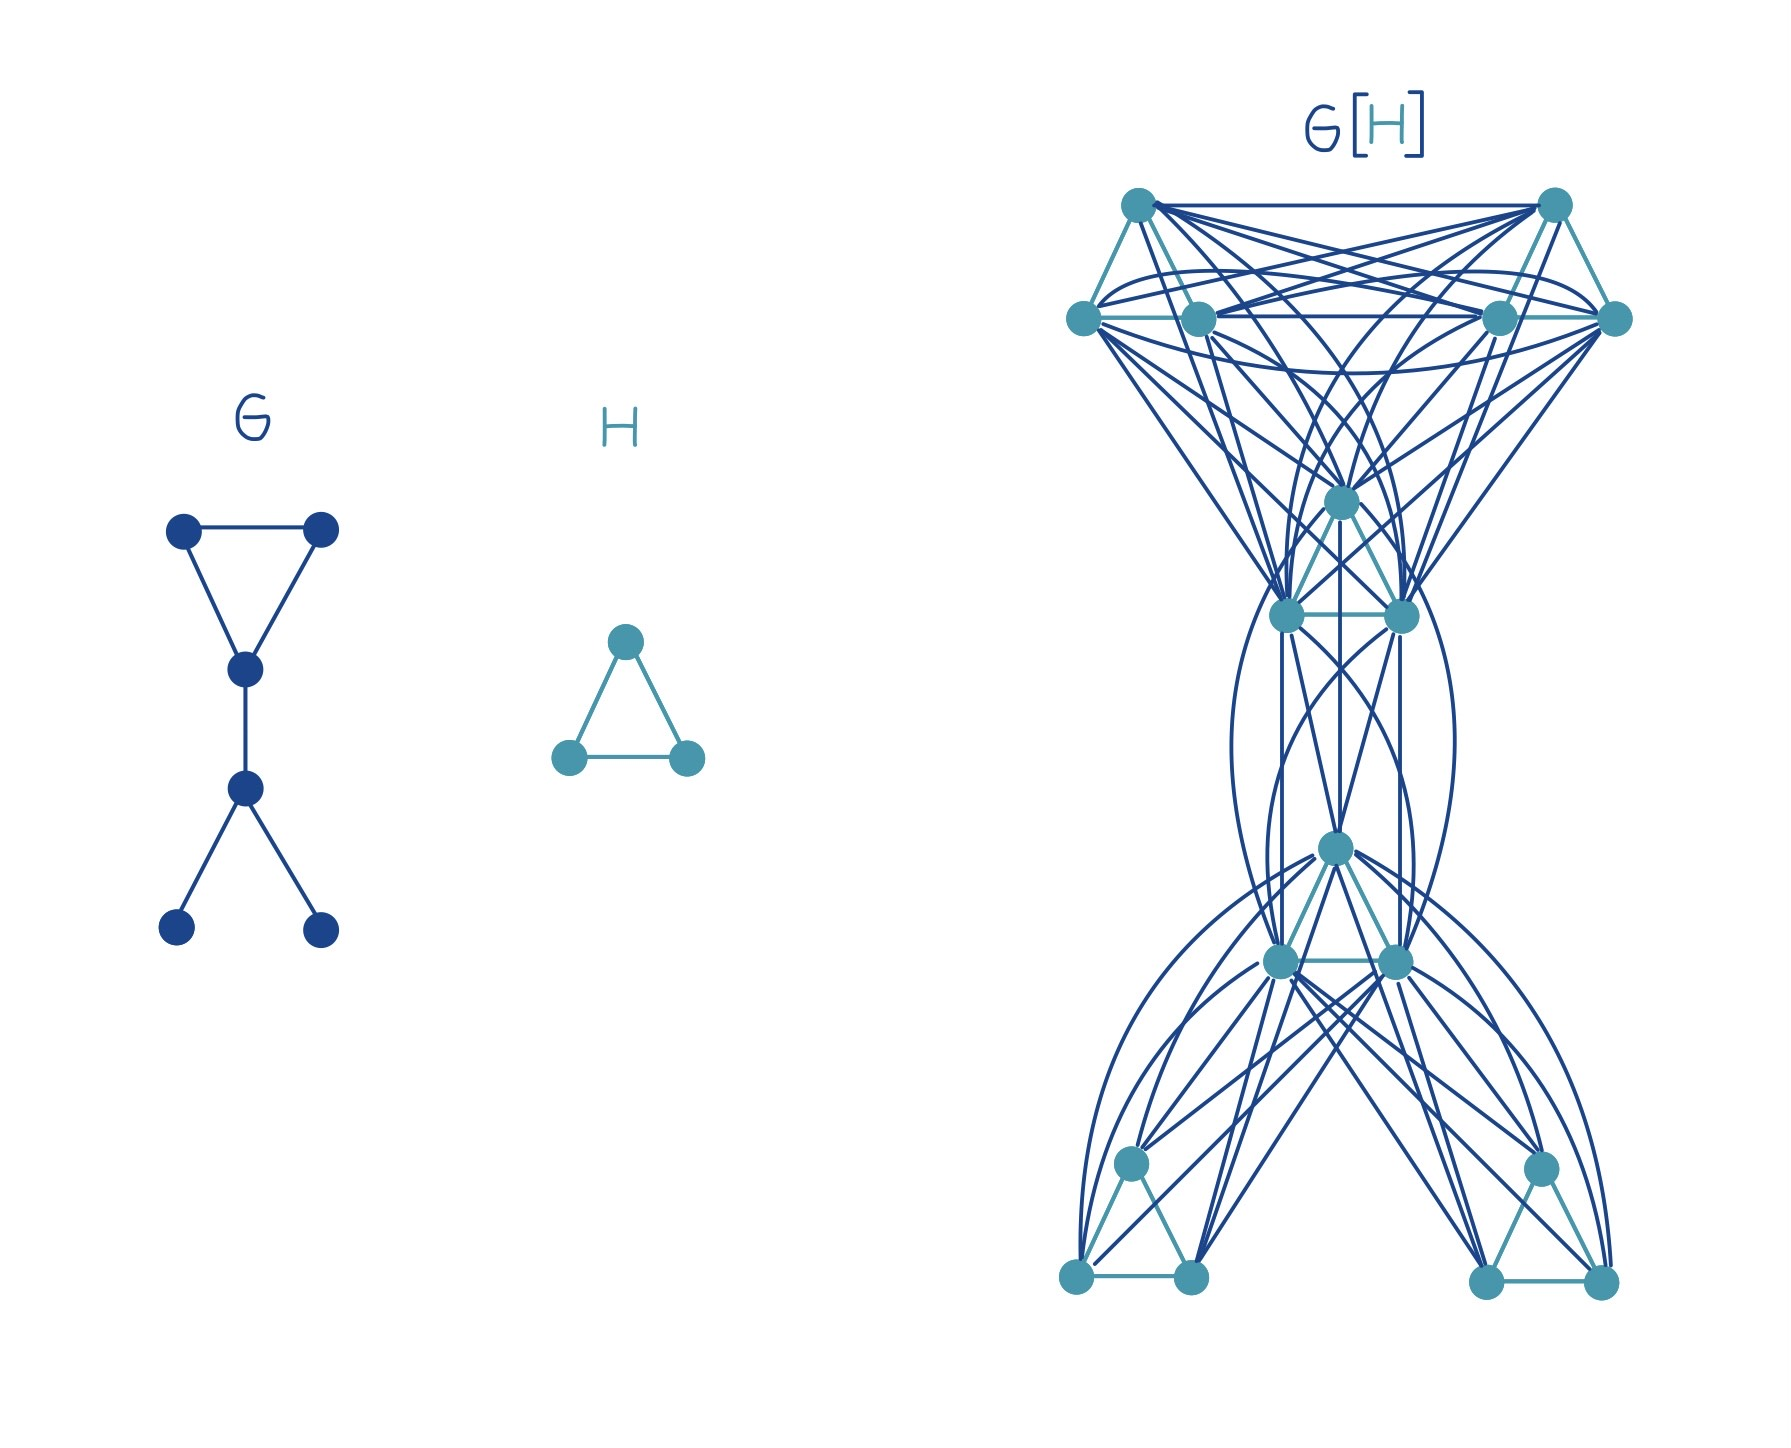
\includegraphics[width=\textwidth]{IMG_produkt.jpg}   
    \caption{Leksikografski produkt povezanih grafov $G$ in $H$.}   
    \label{fig:produkt}
\end{figure}


%%%%%%%%%%%%%%%%%%%%%%%%%%%%%%%%%%%%%%%%%%%%%%%%%%%%%%%%%%%%%%%%%%%%%%%%%%%%%%%
%%%%%%%%%%%%%%%%%%%%%%%%%%%%%%%%%%%%%%%%%%%%%%%%%%%%%%%%%%%%%%%%%%%%%%%%%%%%%%%


\subsection{Lastnosti} \label{ss:lastnosti_leks_prod}
Nekaj osnovnih lastnosti leksikografskega produkta grafov:
\begin{itemize}
    \item RED: $|V(G)| = n$ in $|V(H)| = m \; \Rightarrow |V(G[H])| = n \cdot m.$
    \item POVEZANOST: $G[H]$ je povezan $\Leftrightarrow$ $G$ povezan. 
    \item NEKOMUTATIVNOST: v splošnem velja $G[H] \neq H[G].$
    \item DISTRIBUTIVNOST: $(G_1 + G_2)[H] = G_1[H] + G_2[H],$ 
    \item ENAKOST KOMPLEMENTOV: $\overline{G[H]} = \overline{G} [\overline{H}].$
    % kako bi se v resnici pravilno reklo tej lastnosti\ldots?
    \item PREMER: $$ {\rm diam}(G[H]) =  \begin{cases} 
        {\rm diam}(G); & |V(G)| \geq 2 \\
        {\rm diam}(H); & G = K_1
        \end{cases}$$

\end{itemize}

Poglejmo si, kako izgleda razdalja med vozliščema v leksikografskem produktu grafov. 
Opazujemo leksikografski produkt povezanega grafa $G$ reda $n$, z množico vozlišč
$V(G) = \{v_1, v_2, \ldots , v_n \}$ in grafa $H$ reda $m$, z množico vozlišč 
$V(H) = \{u_1, u_2, \ldots , u_m \}$. Vpeljimo oznako 
$v_{ij} := (v_i, u_j) \in V(G[H]).$
Sedaj lahko zapišemo
\begin{equation} \label{eq:razdalja_produkta}
    d_{G[H]}((v_i, u_j), (v_r, u_s)) = 
    \begin{cases}
        d_G(v_i, v_r); & v_i \neq v_r \\
        a_H(u_j, u_s); & \text{sicer}
    \end{cases}
\end{equation} 

Tu je preslikava $a$ definirana v \eqref{eq:fja_a}.


%%%%%%%%%%%%%%%%%%%%%%%%%%%%%%%%%%%%%%%%%%%%%%%%%%%%%%%%%%%%%%%%%%%%%%%%%%%%%%%
%%%%%%%%%%%%%%%%%%%%%%%%%%%%%%%%%%%%%%%%%%%%%%%%%%%%%%%%%%%%%%%%%%%%%%%%%%%%%%%
%%%%%%%%%%%%%%%%%%%%%%%%%%%%%%%%%%%%%%%%%%%%%%%%%%%%%%%%%%%%%%%%%%%%%%%%%%%%%%%
%%%%%%%%%%%%%%%%%%%%%%%%%%%%%%%%%%%%%%%%%%%%%%%%%%%%%%%%%%%%%%%%%%%%%%%%%%%%%%%


\section{Metrična dimenzija leksikografskega produkta grafov}\label{s:mdim_prod}
% ali lahko namesto 'leksikografskega produkta grafov' pišem kar G[H]?

%%%%%%%%%%%%%%%%%%%%%%%%%%%%%%%%%%%%%%%%%%%%%%%%%%%%%%%%%%%%%%%%%%%%%%%%%%%%%%%
%%%%%%%%%%%%%%%%%%%%%%%%%%%%%%%%%%%%%%%%%%%%%%%%%%%%%%%%%%%%%%%%%%%%%%%%%%%%%%%


\subsection{Metrična dimenzija leksikografskega produkta glede na metrično 
dimenzijo grafa $H$} \label{ss:mdim_komp_prod}

%TA PODNASLOV NI NAJBOLJ POSREČEN
V tem razdelku obravnavamo leksikografski produkt $G[H]$, kjer je $G$ povezan graf reda vsaj $2$ 
in $H$ poljuben graf reda vsaj $2$, ki ima $k\geq 1$ komponent. Za komponente grafa $H$ naj velja:
$$1 \leq |V(H_1)| \leq |V(H_2)| \leq \ldots \leq |V(H_k)|.$$ 
Za poljubni $a \in V(G)$ in $b \in V(H)$ vpeljimo še naslednje oznake:
\begin{itemize}
    \item $H(a) = \{ (a, v) \; | \; v \in V(H) \}$.
    \item $G(b) = \{ (v, b) \; | \; v \in V(G) \}$.
    \item $H_i(a) = \{ (a, v) \; | \; v \in V(H_i) \}$.
\end{itemize}

Vzemimo sosednji vozlišči $a$, $b \in V(G)$. Vemo, da je vsako vozlišče iz $H_j(b)$ 
sosednje vsakemu iz $H_i(a)$ za vse $i, j \in \{1, 2, \ldots k\}$.  
Hitro lahko preverimo, da je inducirani podgraf grafa $G[H]$, kjer vzamemo eno 
vozlišče iz množice $H_j(b)$ in vsa vozlišča iz $H_i(a)$, izomorfen grafu $H_i + K_1.$ 
V nadaljevanju bomo pokazali, da lahko z metrično dimenzijo tega spoja grafov
navzgor omejimo metrično dimenzijo $G[H]$. Navzdol pa jo bomo omejili s pomočjo sledečih trditev.

\begin{lema} \label{lema:1}
    Naj bosta $a, b \in V(G)$ različna. Potem velja 
    \begin{enumerate}
        \item $\forall x, y \in H(a) \; \forall z \in H(b): d_{G[H]}(x,z) = d_{G[H]}(y,z),$
        \item Naj bo $l \neq i$ in $l \neq j$, potem velja 
        $\forall x \in H_i(a), \; y \in H_j(a) \; \forall z \in H_l(a): d_{G[H]}(x,z) = d_{G[H]}(y,z).$
    \end{enumerate}
\end{lema}

\begin{dokaz}
    Pokažimo vsako točko posebej.
    \begin{enumerate}
        \item Označimo $x = (a, u_i), \; y = (a, u_j), \; z = (b, u_k)$ za neke 
        $u_i, u_j, u_k \in V(H)$.
        Ker je $a \neq b$, po \eqref{eq:razdalja_produkta} sledi 
        $d_{G[H]}((a, u_i), (b, u_k)) = d_G(a, b) = d_{G[H]}((a, u_j), (b, u_k))$. 
        \item Označimo $x = (a, u_i), \; y = (a, u_j), \; z = (a, u_l)$ za neke 
        $u_i \in V(H_i), \; u_j \in V(H_j), \; u_l \in V(H_l)$.
        Po \eqref{eq:razdalja_produkta} sledi $d_{G[H]}((a, u_i), (a, u_l)) = 
        a_H(u_i, u_k) = 2 = a_H(u_j, u_k)= d_{G[H]}((a, u_j), (a, u_k))$.
    \end{enumerate} 
 \end{dokaz}


\begin{trditev} \label{trditev:mbaza_presek}
    Naj bo $W$ metrična baza grafa $G[H]$. Označimo $W_i(a) = W \cap H_i(a)$. Potem 
   $$\forall a \in V(G) \; \forall i \in \{1, 2, \ldots, k\} : V(H_i) \geq 2 \Rightarrow W_i(a) \neq \emptyset.$$
   Velja še več, $|W_i(a)| \geq \beta(H_i).$
\end{trditev}

\begin{dokaz}
    Denimo, da obstaja $a \in V(G)$ za kateterega obstaja tak $i \in \{1, 2, \ldots, k\}$, da je
    $V(H_i) \geq 2$ in velja $ W_i(a) = \emptyset$. Potem obstajata vsaj dve vozlišči iz $x, y \in H_i(a)$ z različnimi
    metričnimi predstavitvami glede na $W$, torej mora obstajati vsaj en $z \in W$, da bo $d_{G[H]}(x, z) \neq d_{G[H]}(x,z).$ 
    To pa je v protislovju s \ref{lema:1}, saj je $z$ bodisi iz $H(b)$ za nek $b \neq a$ bodisi iz $H_j(a)$ za nek $i\neq j$.

    Označimo sedaj $W_i(a) = \{ (a, u_1), (a, u_2), \ldots , (a, u_t)\}$ in denimo, da je $t \leq \beta(H_i).$
    Oglejmo si množico $S = \{u_1, u_2, \ldots, u_t\},$ ki je podmnožica $V(H_i).$ Ker je $|S| \leq \beta(H_i),$
    obstajata dve voizlišči v $H_i$, ki imata enako metrično predstavitev glede na $S$. Označimo ti dve vozlišči
    z $x$ in $y$. Velja torej $d_{H_i}(x, u_i) = d_{H_i}(y, u_i)$ za vsak $u_i \in S$. Potem sledi tudi
    $a_{H_i}(x, u_i) = a_{H_i}(y, u_i)$ in lahko zapišemo:
    $$d_{G[H]}((a, x), (a, u_i)) = a_H(x, u_i) = a_H(y, u_i) = d_{G[H]}((a, y), (a, u_i))$$ za vsak $u_i \in S.$
    To pa je v protislovju s tem, da so vozlišča $(a, u_i)$ vsebovana v metrični bazi $W$.
\end{dokaz}


\begin{trditev}\label{trditev:mbaza_vsebovanost_vozlisc_iz_komponent_H}
    Naj bo $W$ metrična baza grafa $G[H]$. Označimo $W(a) = W \cap H(a).$ Naj ima $H$ $m$
    komponent z enim samim vozliščem, označimo jih $H_1, H_2, \ldots, H_m$. Potem $W(a)$ vsebuje vsaj $m-1$ 
    vozlišč iz unije $ S = H_1(a) \cup H_2(a) \cup \ldots \cup H_m(a)$.
\end{trditev}

\begin{dokaz}
    Označimo $S = \{(a, v_1), (a, v_2), \ldots, (a, v_m)\}$.
    Denimo, da $W(a) \cap S < m-1$. Potem obstajata vsaj dve vozlišči $(a, v_i), (a, v_j) \in S,$ 
    za kateri obstaja vozlišče $(a, w) \in W(a)$, da je
    $d((a, v_i), (a, w)) \neq d((a, v_j), (a, w)).$  
    Ker so $w, v_i, v_j$ vsi iz različnih komponent $H$, je to v protislovju s \ref{lema:1}.
\end{dokaz}


\begin{lema} \label{lema:2}
    Naj bo $Q$ povezan graf. Obstaja metrična baza $W$ grafa $Q + K_1,$ da je 
    $W \subseteq V(Q).$
\end{lema}

\begin{dokaz}
    Označimo množico vozlišč $V(Q + K_1) = V(Q) \cup \{ u \}.$ Naj bo $W$ 
    metrična baza $Q + K_1$. Če $u \notin W$ je lema dokazana. 
    
    Denimo $u \in W.$ 
    V tem primeru ločimo dve situaciji:
    \begin{enumerate}
        \item $W \setminus \{ u \} = \emptyset$     
        
        Po \ref{trd:mdim_polni_pot} sledi $Q + K_1 = P_n$, to pa je možno le za $Q = K_1$, 
        torej za $n = 2$ po defniniciji spoja grafov v \ref{def:spoj}.
     
        Hitro lahko preverimo, da je metrična baza grafa $P_2$ množica, ki vsebuje enega 
        od robnih vozlišč. Torej bi lahko namesto $v$, vzeli vozlišče, ki sestavlja graf 
        $Q$ in tako dobimo metrično bazo $W \subseteq V(Q).$
        
        \item $W \setminus \{ u \} \not = \emptyset$ 
        
        Označimo $W = \{ v_1, v_2, \ldots , v_k, u\}$ in $B = V(Q + K_1) \setminus W = \{ v_{k+1}, v_{k+2}, \ldots, v_n\}$.
        Želimo si vozlišče $u$ zamenjati z enim vozliščem iz $B$. Po definiciji \ref{def:spoj} vemo, da bo vozlišče
        $u$ imelo metrično predstavitev $r_{W'}(u) = \1$ glede na katerokoli množico $W' \subseteq V(Q).$ 
        Za $i \in \{k+1, k+2, \ldots, n\}$ definirajmo $W_i = W \cup \{v_i\}$ in $B_i = B \setminus \{v_i\}.$
        $u$ torej lahko zamenjamo z drugim vozliščem le, če obstaja vozlišče $v_i \in B$ tako,
        da velja $\forall v_j \in B_i : r_{W_i} (v_j) \neq \1.$ Če tak $v_i$ obstaja, ga 
        zamenjamo z $u$ v $W$ in smo dobili iskano metrično bazo. 
        
        Če tako vozlišče ne obstaja, je $Q + K_1$ poln graf. Za poln graf pa lahko vzamemo
        rešljivo množico, ki vsebuje vse razen enega vozlišča, torej $W = V(Q).$
    \end{enumerate}
\end{dokaz}


\begin{lema} \label{lema:3}
    Naj bo $a \in V(G)$ in $B_i$ metrična baza grafa $H_i + K_1,$ za katero velja $B_i \subseteq V(H_i).$
    Označimo $W_i(a) = \{(a,x) | \; x \in B_i\}$ in $W(a) = \cup_{1 \leq i \leq k} W_i(a)$. 
    Potem sta za $x, y \in V(H)$ ekvivalentni naslednji trditvi:
    \begin{enumerate}
        \item $r_{W(a)}(a, x) = r_{W(a)}(a, y);$
        \item $x \in V(H_i), \; y \in V(H_j), \; r_{B_i}(x) = \2, \; r_{B_j}(y) = \2,$ kjer je $i\neq j.$
    \end{enumerate}
\end{lema}

\begin{dokaz}
    $\Leftarrow$

    Naj bo $x \in V(H_i), \; y \in V(H_j), \; r_{B_i}(x) = \2, \; r_{B_j}(y) = \2,$ kjer je $i\neq j.$ Torej velja:
    \begin{itemize}
        \item $\forall w \in B_i: \; d_{H_i}(x, w) = 2$ in za take $w$ sledi tudi $a_{H_i}(x, w) = 2,$
        \item $\forall w \in B_j: \; d_{H_j}(y, w) = 2$ in za take $w$ sledi tudi $a_{H_j}(y, w) = 2.$
    \end{itemize}
    Hkrati pa je očitno tudi
    \begin{itemize}
        \item $\forall w \in V(H)\setminus V(H_i): \; a_{H}(x, w) = 2$,
        \item $\forall w \in V(H)\setminus V(H_j): \; a_{H}(y, w) = 2$.
    \end{itemize}
    Potem je 
    $$d_{G[H]}((a, x), (a, w)) = a_H(x, w) = 2 = a_H(y, w)= d_{G[H]}((a, y), (a, w))$$
    za vse $(a, w) \in W(a)$ in sledi $r_{W(a)}(a, x) = r_{W(a)}(a, y).$

    $\Rightarrow$
    Naj bosta $x$ in $y$ različna, za katera velja $r_{W(a)}(a, x) = r_{W(a)}(a, y).$ Torej je 
    $$d_{G[H]}((a, x), (a, w)) = a_H(x, w) = a_H(y, w)= d_{G[H]}((a, y), (a, w))$$ za vsak
    $w \in B = B_i \cup B_2 \cup \ldots \cup B_k.$
    Opazimo, da v grafu $H + K_1$ velja $\forall v, u \in V(H): \; d(v,u) = a(v, u).$

    Naj bo $x \in V(H_i).$ Potem je očitno $\forall w \in B\setminus B_i: a_H(x, w) = 2 = a_H(y, w).$
    Preveriti moramo še vozlišča iz $B_i.$
    \begin{enumerate}
        \item Denimo, da $\exists w_i \in B_i: \; a_H(x, w_i) = 0 \Rightarrow a_H(y,w_i) = 0$ in $x = y$, kar je prostislovje.
        \item Denimo, da $\exists w_i \in B_i: \; a_H(x, w_i) = 1 \Rightarrow a_H(y,w_i) = 1 \Rightarrow y \in V(H_i),$ to pa je 
        protislovju s predpostavko. Ker je $B_i$ baza $H_i + K_1,$ bi moralo veljati 
        $d_{H_i + K_1}(x, b) = a_H(x, b) \neq a_H(y, b) = d_{H_i + K_1}(y, b)$ 
        za vsaj en $b \in B_i$.
    \end{enumerate}
    Sledi $\forall w \in B: \; a_H(x, w) = 2 = a_H(y, w)$ in $r_{B_i}(x) = \2 = r_{B_j}(y).$
\end{dokaz}

TU ŠE LEMA DA JE w(A) = w PRESEK h(A) BAZA ZA h(A).
+ POPRAVI OZNAKE h(A) NAJ BO INDUCIRAN PODGRAF, MEDTEM KO v(h(A)) MNOZICA VOZLIŠČ.

\begin{lema} \label{lema:4}
    Naj bo $a \in V(G)$ in $W$ metrična baza grafa $G[H].$ Označimo $W(a) = W \cap H(a).$ Potem velja:
    $$|W(a)| \leq \Bigl ( \sum_{p=1}^{k} \beta(H_p + K_1) \Bigr ) + k - 1.$$
\end{lema}

TEGA DOKAZA NE RAZUMEM

\begin{dokaz}
    Naj bodo za vsak $i = 1, 2, \ldots, k$ $B_i$ metrična baze $H_i + K_1,$ takšna, da je $B_i \subseteq V(H_i).$ 
    Ta obstaja po \ref{lema:2}. Označimo $W_i(a) = \{(a,x) | \; x \in B_i\}$ in $\widetilde{W}(a) = \cup_{1 \leq i \leq k} W_i(a)$.
    Ločimo dva primera.
    \begin{enumerate}
        \item Denimo, da ne obstajata taka $x \in V(H_i)$ in $y\in V(H_j),$ ki bi zadoščala \ref{lema:3}.
        Torej velja $r_{\widetilde{W}(a)}(a, x) \neq r_{\widetilde{W}(a)}(a, y)$ za vse $(a, x), (a, y) \in H(a)$.
        To pomeni, da je $\widetilde{W}(a)$ rešljiva za $H(a).$ Sledi
        $$|W(a)| \leq |\widetilde{W}(a)| = \sum_{i = 1}^{k} |W_i(a)| = \sum_{i = 1}^{k} |B_i| = \sum_{i = 1}^{k} \beta(H_i + K_1).$$
        \item Demimo, da obstajata taka $x \in V(H_i)$ in $y\in V(H_j),$ ki zadoščata \ref{lema:3}.
        Označimo $S =\{(a, x) \; | \; x \in V(H_i), r_{B_i}(x) = \2 \}$. Opazimo, da je $|S| \leq k,$ saj je v vsaki množici $V(H_i)$
        največ eno tako vozlišče, sicer $B_i$ ne bi bila metrična baza za $H_i + K_1$. Po \ref{trd:cela_resljiva} lahko izberemo 
        $\widetilde{S} = S \setminus \{z\}$ za nek $z \in S$ in vemo, da je $\widetilde{S}$ rešljiva za $S$. $W_i(a)$ je rešljiva za $H_i(a)$
        in sledi, da je $\widetilde{W}(a) \cup \widetilde{S}$ rešljiva za $H(a).$ Velja
        $$|W(a)| \leq |\widetilde{W}(a) \cup \widetilde{S}|  \leq |\widetilde{W}(a)| +  |\widetilde{S}| \leq 
        \Bigl ( \sum_{p=1}^{k} \beta(H_p + K_1) \Bigr ) + k - 1. $$
        
    \end{enumerate}
\end{dokaz}


Vzemimo dve vozlišči $u, v \in V(G)$ in definirajmo množico, ki vsebuje vse najkrajše poti med njima: 
$$P(u,v) = \{w \in V(G) | w \; \text{del katere od najkrajših poti med $u$ in $v$}\}.$$
Naj bo $z\in V(G) \setminus P(u,v).$ Če velja $d(u, v) + d(v, z) > d(u, z)$ in $d(u, v) + d(u, z) > d(v, z)$
 potem je vsaka pot med $u$ in $v$ iz $P(uv)$ ekscentrična. 


\begin{lema} \label{lema:5}
    Naj bodo $a, b \in V(G)$. Označimo $W = \cup_{a \in V(G)} W(a),$ kjer je $W(a)$ metrična baza za graf 
    $H(a)$. Potem za $x, y \in V(H)$ velja:
    $$r_W(a, x) = r_W(b, y) \Leftrightarrow r_{W(a)}(a,x) = \2, \; r_{W(b)}(b,y) = \2$$ in je vsaka najkrajša pot med
    $a$ in $b$ v $G$ ekcentrična pot dolžine $2$.
\end{lema}

\begin{dokaz}
TODO    
\end{dokaz}


\begin{trditev} \label{trditev:zgornja_meja_mdim_leksp}
    Velja
    $$\beta(G[H]) \leq 
    n \cdot \Bigl ( \Bigl ( \sum_{p=1}^{k} \beta(H_p + K_1) \Bigr ) + k - 1  \Bigr ) + (n-2). $$
\end{trditev}

\begin{dokaz}
    Naj bo $a \in V(G)$, $W(a)$ metrična baza za $H(a)$ in definirajmo $W = \cup_{a \in V(G)} W(a).$
    Ločimo dva primera.
    \begin{enumerate}
        \item Denimo, da za vse $x, y \in V(H)$ in $b \in V(G)$ velja $r_W(a, x) \neq r_W(b, y).$ To 
        pomeni, da je $W$ rešljiva za $G[H]$. 
        Torej je ob upoštevanju \ref{lema:4}
        $$\beta(G[H]) \leq |W| = \sum_{a \in V(G)} |W(a)| = n \cdot |W(a)| \leq n \cdot \Bigl ( \sum_{p=1}^{k} \beta(H_p + K_1) \Bigr ) + k - 1.$$
        \item Naj obstajajo 
    \end{enumerate}
\end{dokaz}

\begin{izrek} \label{izrek:omejitve_mdim_komp}
    Naj bo $G$ povezan graf reda $n \geq 2$ in $H$ poljuben graf reda $m \geq 2$, s $k \geq 1$ 
    komponentami $H_1, H_2, \ldots , H_k$. Potem velja:
    $$
    n \cdot \Bigl ( \Bigl ( \sum_{p=1}^{k} \beta(H_p) \Bigr )  - 1  \Bigr ) 
    \leq \beta(G[H]) \leq 
    n \cdot \Bigl ( \Bigl ( \sum_{p=1}^{k} \beta(H_p + K_1) \Bigr ) + k - 1  \Bigr ) + (n-2). 
    $$
\end{izrek}
\begin{dokaz}

\end{dokaz}


%%%%%%%%%%%%%%%%%%%%%%%%%%%%%%%%%%%%%%%%%%%%%%%%%%%%%%%%%%%%%%%%%%%%%%%%%%%%%%%


\subsubsection{H je nepovezan graf} \label{sss:nepovezan}

V dokazu naslednjega izreka bomo konstruirali grafe, katerih metrična dimenzija je enaka
spodnji ali zgornji meji iz izreka \ref{izrek:omejitve_mdim_komp} ter dvema vmesnima vrednostima.
    
\begin{izrek} \label{izrek:primeri_mdim_komp}
Obstajata taka grafa $G$ in $H$, da je $G$ povezan graf reda $n \geq 2$ in $H$ poljuben graf 
reda $m \geq 2$, s $k \geq 1$ komponentami $H_1, H_2, \dots , H_k$, da velja:
    \begin{enumerate}
        \item $\beta(G[H]) = n \cdot \Bigl ( \Bigl ( \sum_{p=1}^{k} \beta(H_p) \Bigr )  - 1  \Bigr )$.
        \item $\beta(G[H]) = n \cdot \Bigl ( \Bigl ( \sum_{p=1}^{k} \beta(H_p + K_1) \Bigr ) + k - 1 
        \Bigr ) + (n-2)$.
        \item $\beta(G[H]) = n \cdot \Bigl ( \Bigl ( \sum_{p=1}^{k} \beta(H_p + K_1) \Bigr ) + k - 1  
        \Bigr )$.
        \item $\beta(G[H]) = n \cdot \Bigl ( \sum_{p=1}^{k} \beta(H_p + K_1) \Bigr ) $.
    \end{enumerate}
\end{izrek}
    
\begin{dokaz}
    \begin{enumerate}
        \item Naj bo $G = P_n$, $n\geq 4$ in $H = N_k$, $k\geq 2$. 
        Zaradi izreka \ref{izrek:omejitve_mdim_komp} je dovolj pokazati 
        $\beta(G[H]) \leq n \cdot \Bigl ( \Bigl ( \sum_{p=1}^{k} \beta(H_p) \Bigr )  - 1  \Bigr ) = n 
        \cdot (k - 1)$. Označimo $V(G) = \{p_1 , p_2, \ldots, p_n\}$, kjer so $\forall 1 \leq i < n : \; 
        p_i p_{i+1} \in E(G)$, in $V(H) = \{ v_1, v_2, \ldots, v_k\}.$ Definirajmo množico 
        $W = V(G[H]) \setminus G(v_k).$ Velja $|W| = n \cdot (k-1).$ 
        Pokažimo, da je $W$ rešljiva množica. Opomba \ref{op:zadostno_preverjanje} nam pove, da je dovolj preveriti
        vozlišča iz množice $G(v_k) = \{ (p_1, v_k), (p_2, v_k), \ldots, (p_n, v_k)\}$. Če se spomnimo formule
        \eqref{eq:razdalja_produkta}, vidimo, da velja:
        \begin{itemize}
            \item $2 \leq d((p_i, v_k), (p_{j+1}, v_1)) \neq d((p_j, v_k), (p_{j + 1}, v_1)) = 1,$ 
            za $ 1 \leq i \leq j < n $.
            \item $2 \leq d((p_n, v_k), (p_{i-1}, v_1)) \neq d((p_i, v_k), (p_{i- 1}, v_1)) = 1,$ 
            za $ 2 \leq i < n $.
            \item $1 = d((p_1, v_k), (p_2, v_1)) \neq d((p_n, v_k), (p_2, v_1)) \geq 2.$
        \end{itemize}
        Sledi, da so metrične predstavitve vozlišč iz $G(v_k)$ paroma različne in je $W$ rešljiva množica.
    
        \item Naj bo $G = S_{n-1}$ zvezda na $n$ vozliščih, $n\geq 4$, in $H$ graf s $k \geq 2$ komponentami
        $H_1, H_2, \ldots, H_k,$ kjer je $H_i = P_8.$ Velja $\beta(P_8 + K_1) = 
        \Bigl \lfloor \frac{2\cdot 8 + 2}{5} \Bigr \rfloor = 3. $ % DOKAZ??
        Zato je, podobno kot v prvi točki, dovolj pokazati  
        $$\beta(G[H]) \geq n \cdot \Bigl ( \Bigl ( \sum_{p=1}^{k} \beta(H_p + K_1) \Bigr ) + k - 1 \Bigr ) + 
        (n-2) = 4kn - 2.$$ 
        Naj bo $B$ metrična baza $P_8 + K_1$, potem obstaja $v \in V(P_8),$ da je $r_B(v) = (2, 2, 2).$
            %DOKAZ??
    
        Recimo, da je $\beta(G[H]) < 4kn - 2,$ in naj bo $W$ metrična baza $G[H]$. 
            
        TODO
    
        \item TODO
        \item TODO
    
    \end{enumerate}
\end{dokaz}


%%%%%%%%%%%%%%%%%%%%%%%%%%%%%%%%%%%%%%%%%%%%%%%%%%%%%%%%%%%%%%%%%%%%%%%%%%%%%%%


\subsubsection{H je povezan graf} \label{sss:povzean}


\begin{izrek} \label{izrek:primeri_mdim_komp_povezan}
    Naj bo $G$ povezan graf reda $n \geq 2$ in $H$ povezan graf reda $m \geq 2$. Potem velja:
    $$
    n \cdot \beta(H)  
    \leq \beta(G[H]) \leq 
    n \cdot \beta(H_p + K_1) + (n-2). 
    $$
\end{izrek}

\begin{izrek} \label{izrek:omejitve_mdim_komp_povezan}
    Obstajata taka grafa povezana $G$ in $H$, reda vsaj $2$, da velja:
    \begin{enumerate}
        \item $\beta(G[H]) = n \cdot \beta(H)$
        \item $\beta(G[H]) = n \cdot \beta(H_p + K_1) + (n-2)$
        \item $\beta(G[H]) = n \cdot \beta(H_p + K_1)$
    \end{enumerate}
\end{izrek}
    
\begin{dokaz}
    TODO
\end{dokaz}

Na tej točki se lahko vprašamo, če za vsako vrednost $c$ znotraj zgornjih mej lahko najdemo
grafa $G$ in $H$, ki bosta zadoščala $\beta(G[H]) = c$.

%%%%%%%%%%%%%%%%%%%%%%%%%%%%%%%%%%%%%%%%%%%%%%%%%%%%%%%%%%%%%%%%%%%%%%%%%%%%%%%
%%%%%%%%%%%%%%%%%%%%%%%%%%%%%%%%%%%%%%%%%%%%%%%%%%%%%%%%%%%%%%%%%%%%%%%%%%%%%%%


\subsection{Metrična dimenzija, sosedska dimenzija in dvojčki}
V tem podpoglavju bomo obravnavali metrično dimenzijo leksikografskega produkta $G[H]$ na 
podlagi reda grafa $G$ in sosedske dimenzije grafa $H$. 

\begin{lema}
    Naj bo $G$ povezan graf reda $n$ in $H$ poljuben graf. Potem velja:
    $$\beta(G[H]) \geq n \cdot \mu(H).$$
\end{lema}

\begin{dokaz}
    TODO
\end{dokaz}


\begin{trditev}
    Naj bo $G$ povezan graf reda $n$ in $H$ poljuben graf. Če obstajata dve sosedski bazi 
    grafa $H$, $S_1$ in $S_2$, da nobeno vozlišče nima sosedske predstavitve z množico $S_1$ 
    enako $\1$ in nobeno vozlišče nima sosedske predstavitve z množico $S_2$ 
    enako $\2$, potem velja $$\beta(G[H]) = \beta(G[\overline{H}]) = n \cdot \mu(H). $$
\end{trditev}

\begin{dokaz}
    TODO
\end{dokaz}


\begin{trditev}
    Naj bo $G$ povezan graf reda $n$ in $H$ poljuben graf. Če za vsako sosedsko bazo $S$
    grafa $H$ obstajata vozlišči s sosedskima predstavitvama glede na $S$ enakima $\1$ in $\2$,
    potem je 
    $$\beta(G[H]) = \beta(G[\overline{H}]) = n \cdot (\mu(H) + 1) - \iota(G). $$
\end{trditev}

\begin{dokaz}
    TODO
\end{dokaz}


\begin{trditev}
    Naj bo $G$ povezan graf reda $n$ in $H$ poljuben graf. Naj ima $H$ sledeči lastnosti:
    \begin{enumerate}
        \item za vsako sosedsko bazo obstaja vozlišče s sosedsko predstavitvijo $\1$,
        \item obstaja sosedska baza $S$, da nobeno vozlišče nima sosedske predstavitve enake $\2.$
    \end{enumerate} 
    Potem velja $$\beta(G[H]) = n \cdot \mu(H) + a(G) - \iota_K(G). $$
\end{trditev}

\begin{dokaz}
    TODO
\end{dokaz}


\begin{trditev}
    Naj bo $G$ povezan graf reda $n$ in $H$ poljuben graf. Naj ima $H$ sledeči lastnosti:
    \begin{enumerate}
        \item za vsako sosedsko bazo obstaja vozlišče s sosedsko predstavitvijo $\2$,
        \item obstaja sosedska baza $S$, da nobeno vozlišče nima sosedske predstavitve enake $\1.$
    \end{enumerate} 
    Potem velja $$\beta(G[H]) = n \cdot \mu(H) + b(G) - \iota_N(G). $$
\end{trditev}

\begin{dokaz}
    TODO
\end{dokaz}


\begin{izrek}
    Če je $G$ povezan graf reda $n$, ki nima dvojčkov, velja $\beta(G[H]) = n \cdot \mu(H).$
\end{izrek}

\begin{dokaz}
    Če $G$ nima dvojčkov, je $\iota(G) = n$, $\iota_K(G) = a(G) = 0$ in $\iota_N(G) = b(G) = 0.$
    Graf $H$ gotovo zadostuje pogojem v eni od zgornjih treh trditev, zato sledi  
    $\beta(G[H]) = n \cdot \mu(H).$
\end{dokaz}


\begin{izrek}
    Naj bo $G = P_n$, za $n\geq 4$ ali $G = C_n$ za $n \geq 5,$ ter naj bo $m\geq 3.$ Tedaj velja
    $\beta(G[P_m]) = \beta(G[C_m]) = \beta(G[\overline{P_m}]) = \beta(G[\overline{C_m}]) = 
    n \cdot  \Bigl \lfloor \frac{2\cdot m + 2}{5} \Bigr \rfloor $.

    Velja še več, 
    $$\beta(G[K_{m_1, \ldots, m_t}]) = \beta(G[\overline{K}_{m_1, \ldots, m_t}]) = 
    \begin{cases}
        n \cdot (m - r - 1); & r \neq t, \\
        n \cdot (m - r); & r = t, 
    \end{cases} $$
    kjer so $m_1, \ldots, m_r \geq 2$,  $m_{r+1} = \ldots = m_t = 1$ in $\sum_{i= 1}^{t} m_i = m.$
\end{izrek}

\begin{dokaz}
    TODO
\end{dokaz}

\begin{izrek}
    Naj bodo $n, m, m_1, \ldots, m_t$ števila, za katera velja:
    \begin{itemize}
        \item $n \geq 2$,
        \item $m_1, \ldots, m_r \geq 2$,
        \item $m_{r+1} = \ldots = m_t = 1$,
        \item $\sum_{i= 1}^{t} m_i = m.$.
    \end{itemize}
    Potem velja
    $$\beta(K_n[K_{m_1, \ldots, m_t}]) = 
    \begin{cases}
        n \cdot (m - r) - 1; & r \neq t, \\
        n \cdot (m - r); & r = t, 
    \end{cases} $$.
\end{izrek}

\begin{dokaz}
    TODO
\end{dokaz}




%%%%%%%%%%%%%%%%%%%%%%%%%%%%%%%%%%%%%%%%%%%%%%%%%%%%%%%%%%%%%%%%%%%%%%%%%%%%%%%
%%%%%%%%%%%%%%%%%%%%%%%%%%%%%%%%%%%%%%%%%%%%%%%%%%%%%%%%%%%%%%%%%%%%%%%%%%%%%%%
%%%%%%%%%%%%%%%%%%%%%%%%%%%%%%%%%%%%%%%%%%%%%%%%%%%%%%%%%%%%%%%%%%%%%%%%%%%%%%%
%%%%%%%%%%%%%%%%%%%%%%%%%%%%%%%%%%%%%%%%%%%%%%%%%%%%%%%%%%%%%%%%%%%%%%%%%%%%%%%


\section{Zaključek}
%...
\printbibliography

\end{document}
